\section{Question 2:Parameter Selection and Classification (for dataset B)}
\subsection{Data preprocessing}
Z-score normalization was used for normalizing data instead of the min-max normalization. The Z-Score normalization is a standardization and re-scaling the range of the data in which the mean is centered on zero and it has a unit variance. This means that z-score will still preserve the range of the data (maximum and minimum) as min-max normalization but also will provide the standard deviation and variance of the distribution. This is helpful when it comes for dealing with data flowing in real time as we can easily normalize data coming in using the mean and variance, however, if we used min-max normalization then we might run into an issue where the data coming in is larger than the max the we trained model. This is an advantage that we get by choosing the z-score over the min-max. \\
We split the test and training set randomly in order to evaluate the performance of the models (Classifiers). \\
For this dataset, the distribution of the labels is almost the same. We have 1137 samples labeled as 1 and 1063 samples labeled as -1.


\\
\subsection{Parameter selection:}
\subsubsection{Parameter selection for k-NN}

A k-NN classifier was employed to predict the labels of the data in data set B based on the input of the 56 features. The main hyper parameter of the k-NN model is the number of neighbours, "k". A set of possible values for the hyper parameter were tested and validated using 5 fold cross validation. Each fold represents a slice of the data and one fold at a time is used as the validation set to verify the performance of the model. This model was not validated directly on the test set because 5 fold cross validation intentionally using one of the folds as a test set. In the case of 5 fold the resulting test train split is effectively 80/20. The test set can then be used to compared different models with equal fairness knowing that none of the data would bleed through during the cross validation step.

For each value of K the cross validated accuracy score was returned as the key performance metric. Figure~\ref{fig:knntuning} shows the plot of the accuracy vs the value  of the parameter "k". We see that the model performed best when the value of "k" was set to 15.

\clearpage{}
\begin{figure}[!ht]
 \centering
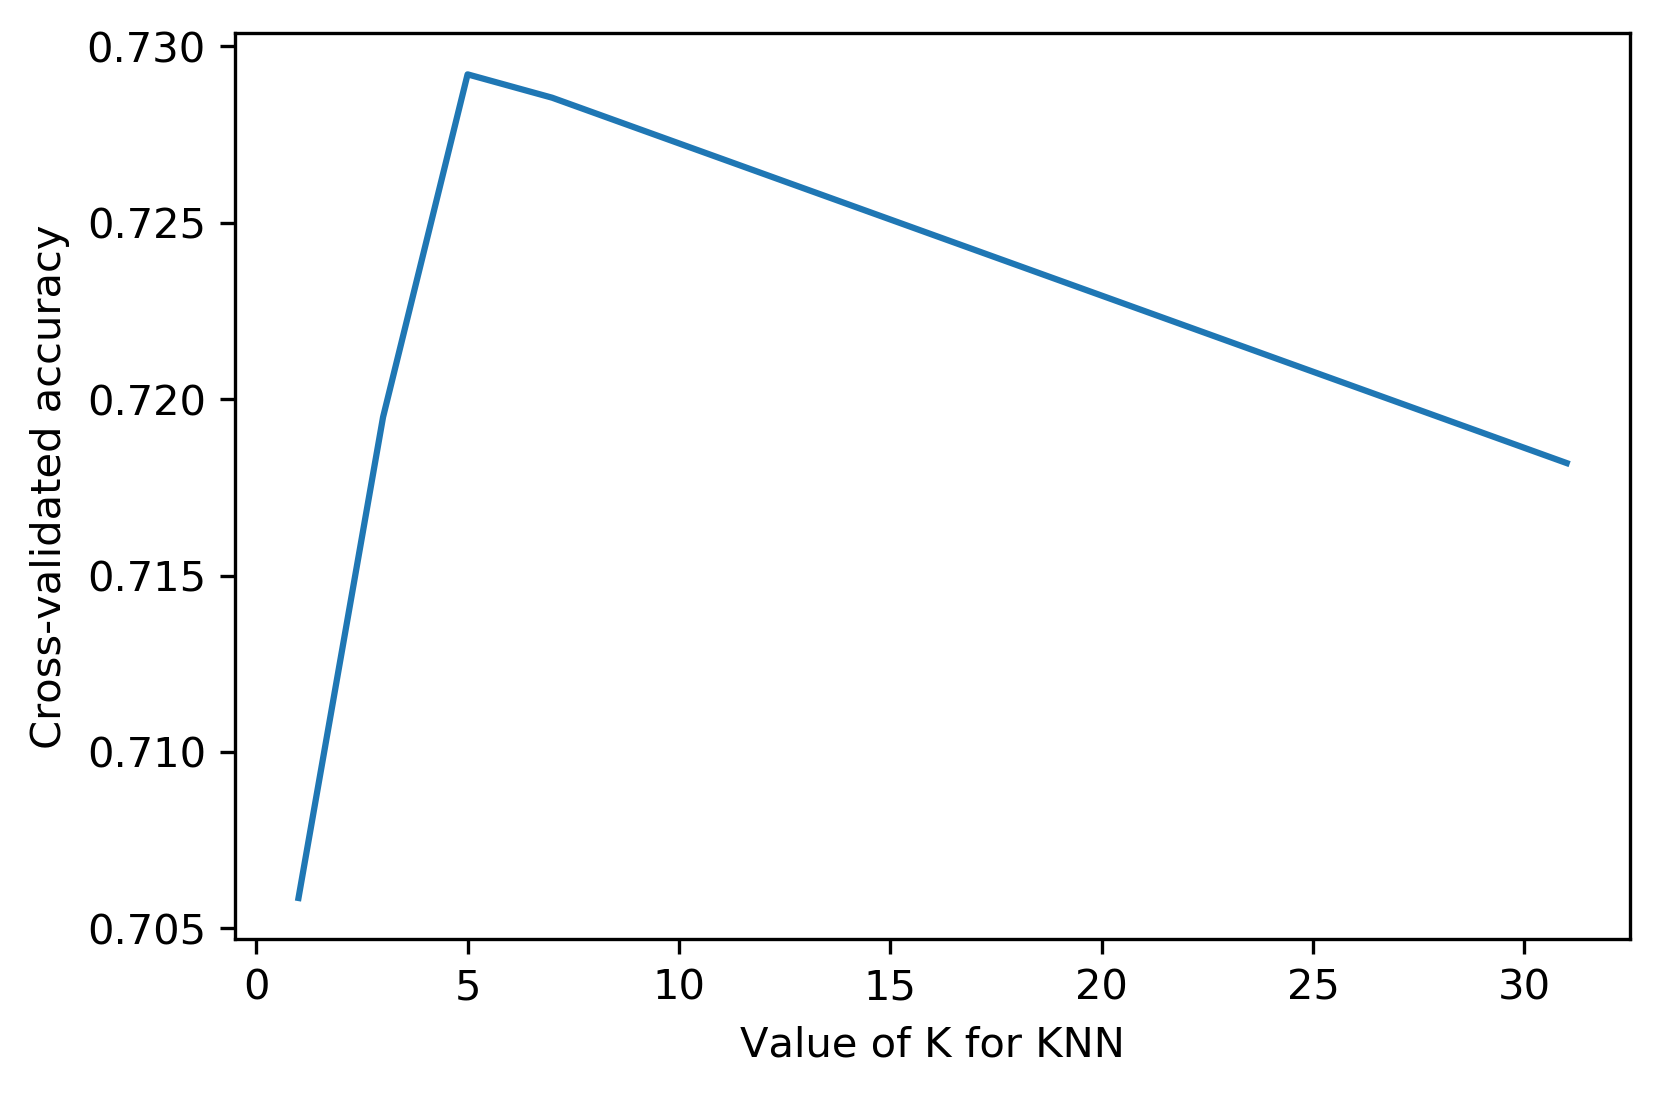
\includegraphics[width=6.1in]{assignment2/2-2-a-kNN.png}
\caption{\label{fig:knntuning} Relationship between accuracy and the parameter k }
\end{figure}



\subsubsection{Parameter selection for SVM}

A support vector machine model was created to predict labels of the given data set. There were two hyper parameters that need to be determined for the SVM model, "C" and "gamma". In order to determine the optimal values a grid search was done over the parameter space with the given set of values. The scoring metric used for each combination of parameters was "roc_auc". The result of the hyper parameter tuning was a value of 0.01 for gamma and 10 for C.

The model was then trained on the training data using the hyper parameters found during the cross validation grid search. Figure~\ref{fig:svmtuning} shows the plot of AUCROC for the tuned and trained SVM model. The AUC of the model is 0.97.


\begin{figure}[!ht]
 \centering
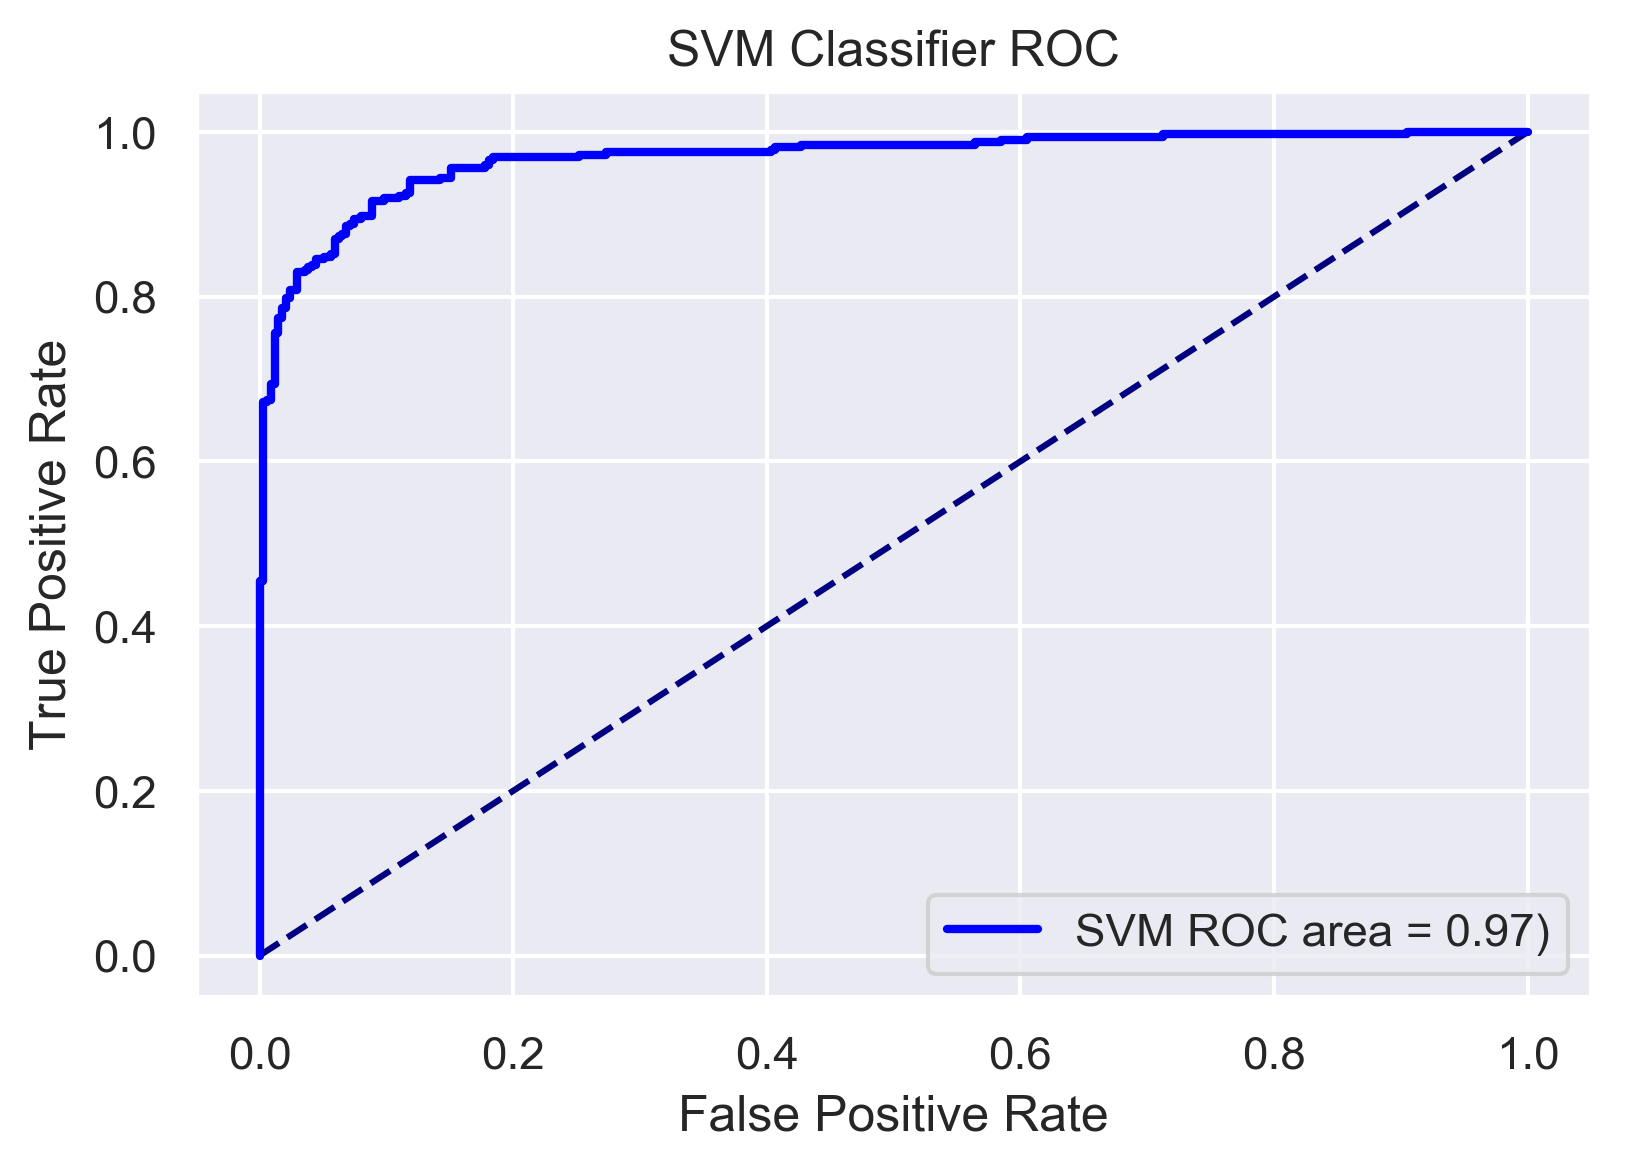
\includegraphics[width=6.1in]{assignment2/2-2-b-svm.png}
\caption{\label{fig:svmtuning} SVM area under curve receiver operator characteristic}
\end{figure}


\subsection{Training six classifiers}

\subsubsection{Classify the test set using k-NN, SVM, Random Forests and Neural Networks. Use the chosen parameters from the parameter selection process in question 2 for k-NN and SVM. For the next two classifiers use the default setups listed at the end for Random Forests and Neural Networks}


The performance for the four models (KNN, SVM, Random Forest and Neural Network) was calculated using the sklearn library function "classification\_report". We can see the results of the classification in Figure~\ref{fig:resultsknnsvm} and Figure~\ref{fig:resulstsrfnn} below. From the results we can see that the KNN model performed the worst with an average F1 score of 0.75. The SVM model and Neural Network with default parameters performed similarly with and average f1 score of 0.91 and 0.90 respectively. Finally the random forest model out performed the other models with an average f1 score of 0.95.

It is important to mention that there are multiple metrics that can be used to evaluate the performance of a model on a binary classification problem. Depending on the data provided and the use case of the model some outcomes may be more desired that others. For example the true positive rate may be more important for a bank to determine default likelihood because of the impact to their business if a false negative is provided. Knowing this it may be more important to value recall over precision or vice-versa. The f1-score does a decent job of blending the performance of both scenarios and is therefore used in this report as the general metric to evaluate performance between these models.

Overall there is not much variation between the various scoring metrics. This is most likely due to the fact that the data set provided is fairly balanced. The count of the true labels and false labels is quite similar. If the data was imbalanced techniques could have been used to reduce the impact to the models where labels are biased to the majority class. This problem may have been an issue for the classifiers found in part 1 as there was a large imbalance between the majority and minority classes.

% \clearpage{}
\begin{figure}[!ht]
 \centering
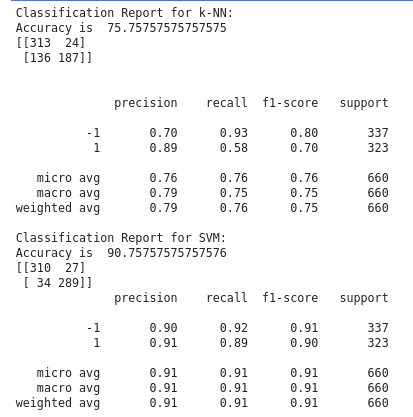
\includegraphics[height=3.5in]{assignment2/2-3-a1.png}
\caption{\label{fig:resultsknnsvm} Performance Result for KNN and SVM models using parameters from section 2.2}
\end{figure}
\clearpage{}
\begin{figure}[!ht]
 \centering
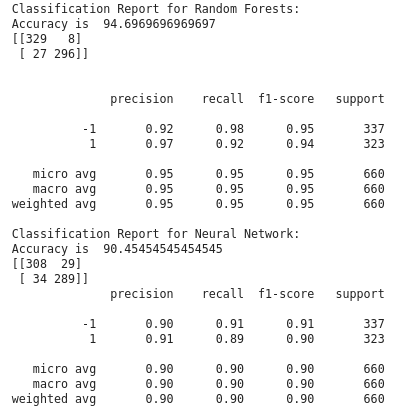
\includegraphics[height=3.5in]{assignment2/2-3-a2.png}
\caption{\label{fig:resulstsrfnn} Performance Result for Random Forest and Neural Network models using default parameters}
\end{figure}


\subsubsection{For the fifth and sixth classifiers, you should explore the parameters of the Random Forests and Neural Network models to devise your own classifier instance that does better than the other methods. For example, you could consider a deeper neural network with multiple layers, use different optimization/solver algorithms, you could modify the Random Forests using different parameter settings for depth and number of trees or enable boosting. Play around with options and choose a setting for RFs and NNs that performs better}

Our first goal is to increase the performance of the random forest model in predicting the test subset of the provided data set. Our approach is to use linear search over two important hyper parameters of the random forest model, "n\_estimators" and "treedepth". Figure~\ref{fig:rfnest} below shows the plot of AUC for both the train and test data. We can see from the plot that the performance of the test AUC starts to decrease when n\_estimators reaches a value greater than 100. Based on this result 100 was chosen for the hyper parameter. 


\begin{figure}[!ht]
 \centering
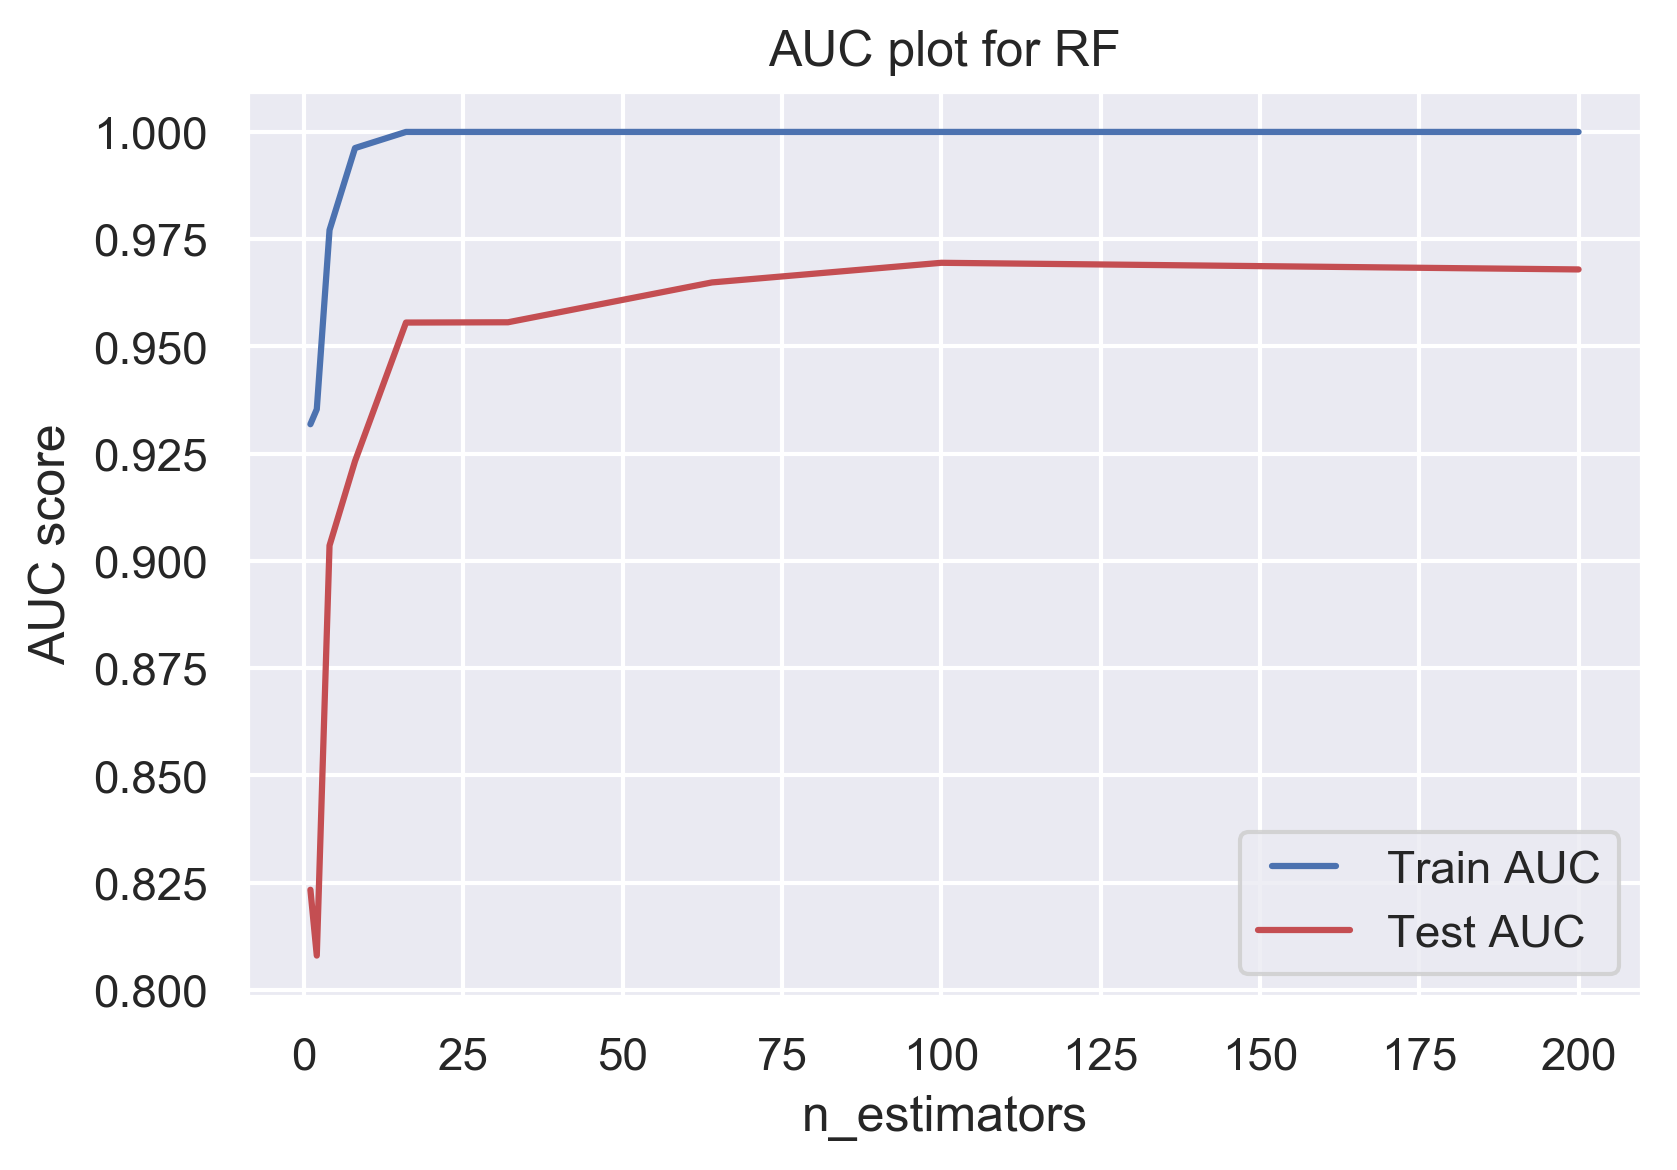
\includegraphics[width=6.1in]{assignment2/2-3-b-rf(n_estimator).png}
\caption{\label{fig:rfnest} Random Forest linear search for optimal n\_estimator parameter value}
\end{figure}

\clearpage{}
Next, a linear search was done to find the optimal value of tree depth. Figure~\ref{fig:rfnest} below shows the plot of AUC vs tree depth. We can see that the test and train data begin to diverge around a tree depth of 5, however test accuracy increases slightly until tree dept is 13. We decided to use a tree depth of 13 for the hyper parameter value.

\begin{figure}[!ht]
 \centering
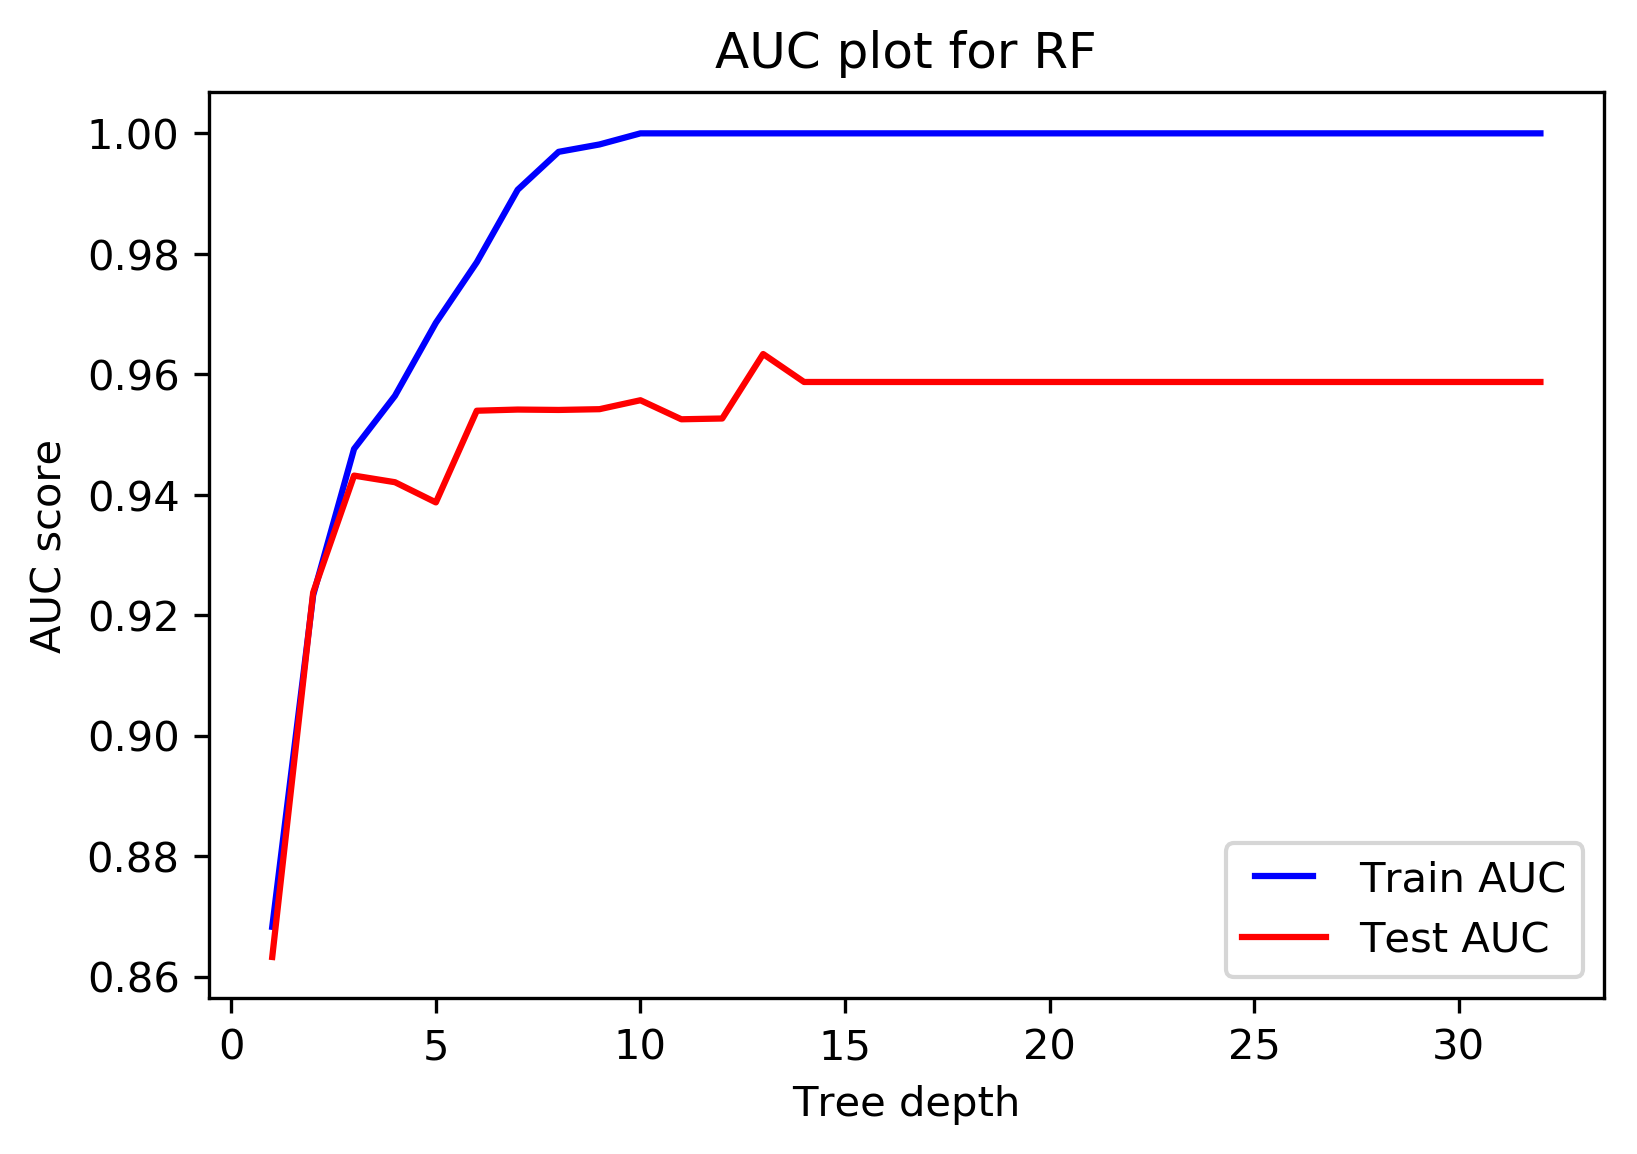
\includegraphics[width=6.1in]{assignment2/2-3-b-rf(Treedepth).png}
\caption{\label{fig:rftreedepth} Random Forest linear search for optimal treedepth parameter value}
\end{figure}




\subsubsection{Repeat each classification method 20 times by varying the split of the training-test set as in question 2-2. Report the average and standard deviation of classification performance on the test set regarding: accuracy, precision, recall, and F- Measure. Also report the training time and classification time of all the methods. Explain why the classification was repeated 20 times}



\subsection{Obtained Results}



\subsection{Feature Removal}
